\documentclass[a4paper,10pt]{article}
\usepackage[utf8]{inputenc}
\usepackage{graphicx}
\usepackage{svg}
\pdfoptionpdfminorversion 6
 
\newcommand{\executeiffilenewer}[3]{%
    \ifnum\pdfstrcmp{\pdffilemoddate{#1}}%
    {\pdffilemoddate{#2}}>0%
    {\immediate\write18{#3}}
    \fi%
}

% includesvg[scale]{file} command (linux-version)
\newcommand{\includesvgcustom}[2][1]{%
  \executeiffilenewer{#2.svg}{#2.pdf}{%
  /usr/bin/inkscape -z -D --file="#2.svg" --export-pdf="#2.pdf" --export-latex}%
  \scalebox{#1}{\input{#2.pdf_tex}}%
}

\begin{document}

\section*{Testing SVG graphics}
\begin{figure}[htbp]
  \centering
  \includesvg[width=0.9\textwidth]{image}
  \caption{This svg image will be embedded using the svg package.}
\end{figure}

%\begin{figure}[htbp]
%  \centering
%  \includesvgcustom[0.8]{image}
%  \caption{This svg image will be converted to PDF on the fly. Scale doesn't work with textwidth.}
%\end{figure}

%\begin{figure}[htbp]
%  \centering
%  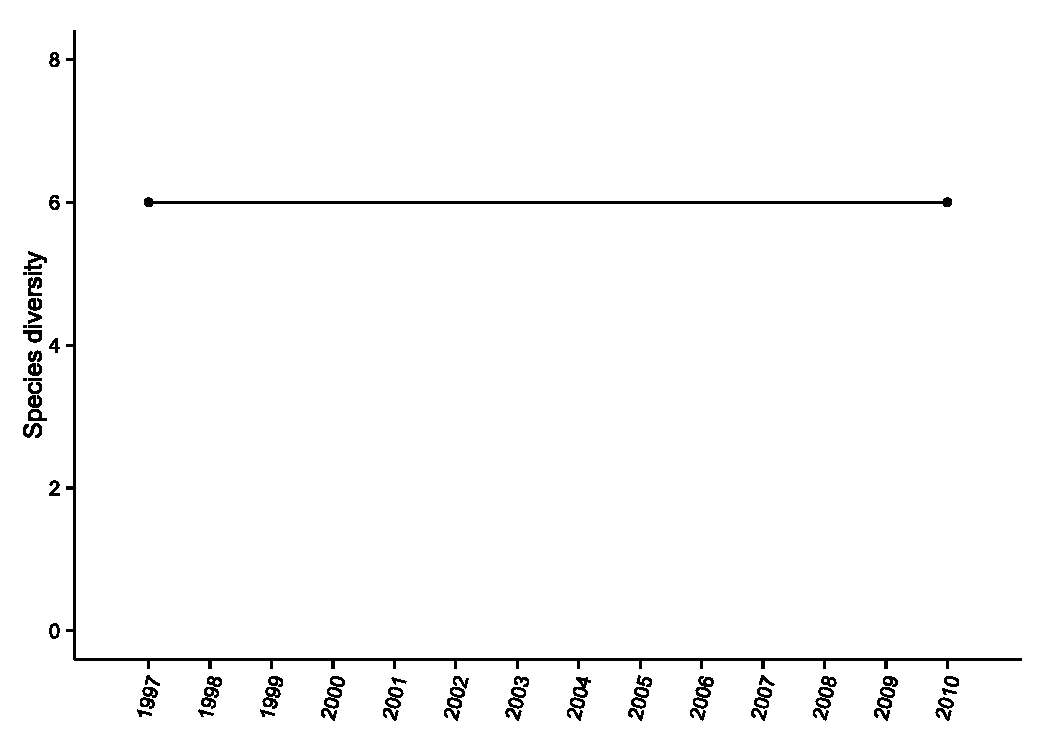
\includegraphics[width=0.9\textwidth]{exported_image.pdf}
%  \caption{This svg image has been converted to PDF using inkscape.}
%\end{figure}

\end{document}
